%!TEX root = main.tex

\section{Numerical experiments} % (fold)
\label{sec:numerical_experiments}

In this section, we present some numerical analyses of our
\emph{Screenkhorn} algorithm and show how it behaves when
integrated into some complex machine learning pipelines.

\subsection{Setup}

We have implemented our Screenkhorn in Python and used the LBFGS of
Scipy. Regarding the machine-learning based comparison, we have based our code
on the ones of POT~\citep{flamary2017pot} and just replaced the Sinkhorn function call with a Screenkhorn one. We have considered the POT's default Sinkhorn stopping criterion parameters and for Screenkhorn, the LBFGS algorithm is stopped when the 
largest component of the projected gradient is smaller than $10^{-6}$, when the number of iterations of number of objective function evaluations reach $10^{5}$. For all applications, we have set $\eta=1$ unless otherwise specified.

\subsection{Analysing on toy problem}

We compare \emph{Screenkhorn} to Sinkhorn as implemented in Python Optimal Transport toolbox\footnote{\url{https://pot.readthedocs.io/en/stable/index.html}} on  a synthetic example. The dataset we use consists of source samples generated from a bi-dimensional gaussian mixture and target samples following the same distribution but with different gaussian means. We consider an unsupervised domain adaptation using optimal transport with entropic regularization.  Several settings are explored: different values of $\eta$, the regularization parameter, the allowed budget $\frac{n_b}{n} = \frac{m_b}{m} = $ ranging from $0.01$ to $0.99$, different values of $n$ and $m$.
% and, whether the cost matrix $C$ is normalized or not.
 We empirically measure  marginal violations as the norms $\norm{{\mu} -{\mu}^{\text{sc}}}_1$ and $\norm{{\nu} -{\nu}^{\text{sc}}}_1$, running time expressed as $\frac{T_{\text{\emph{Screenkhorn}}}}{T_{\text{Sinkhorn}}}$ and the relative divergence difference $| \inr{C, P^\star} - \inr{C, P^{\text{sc}}}|/\inr{C, P^\star}$ between \emph{Screenkhorn} and Sinkhorn, where $P^\star = \Delta(e^{u^\star}) K \Delta(e^{v^\star})$ and $P^{\text{sc}} = \Delta(e^{u^{\text{sc}}}) K \Delta(e^{v^{\text{sc}}}).$

Figure \ref{fig:margin_expe} summarizes the observed behaviors of both algorithms under these settings. We choose to only report results for $n=m=1000$ as we get similar findings for other values of $n$ and $m$. 

\begin{figure*}[t]
	\begin{center}
		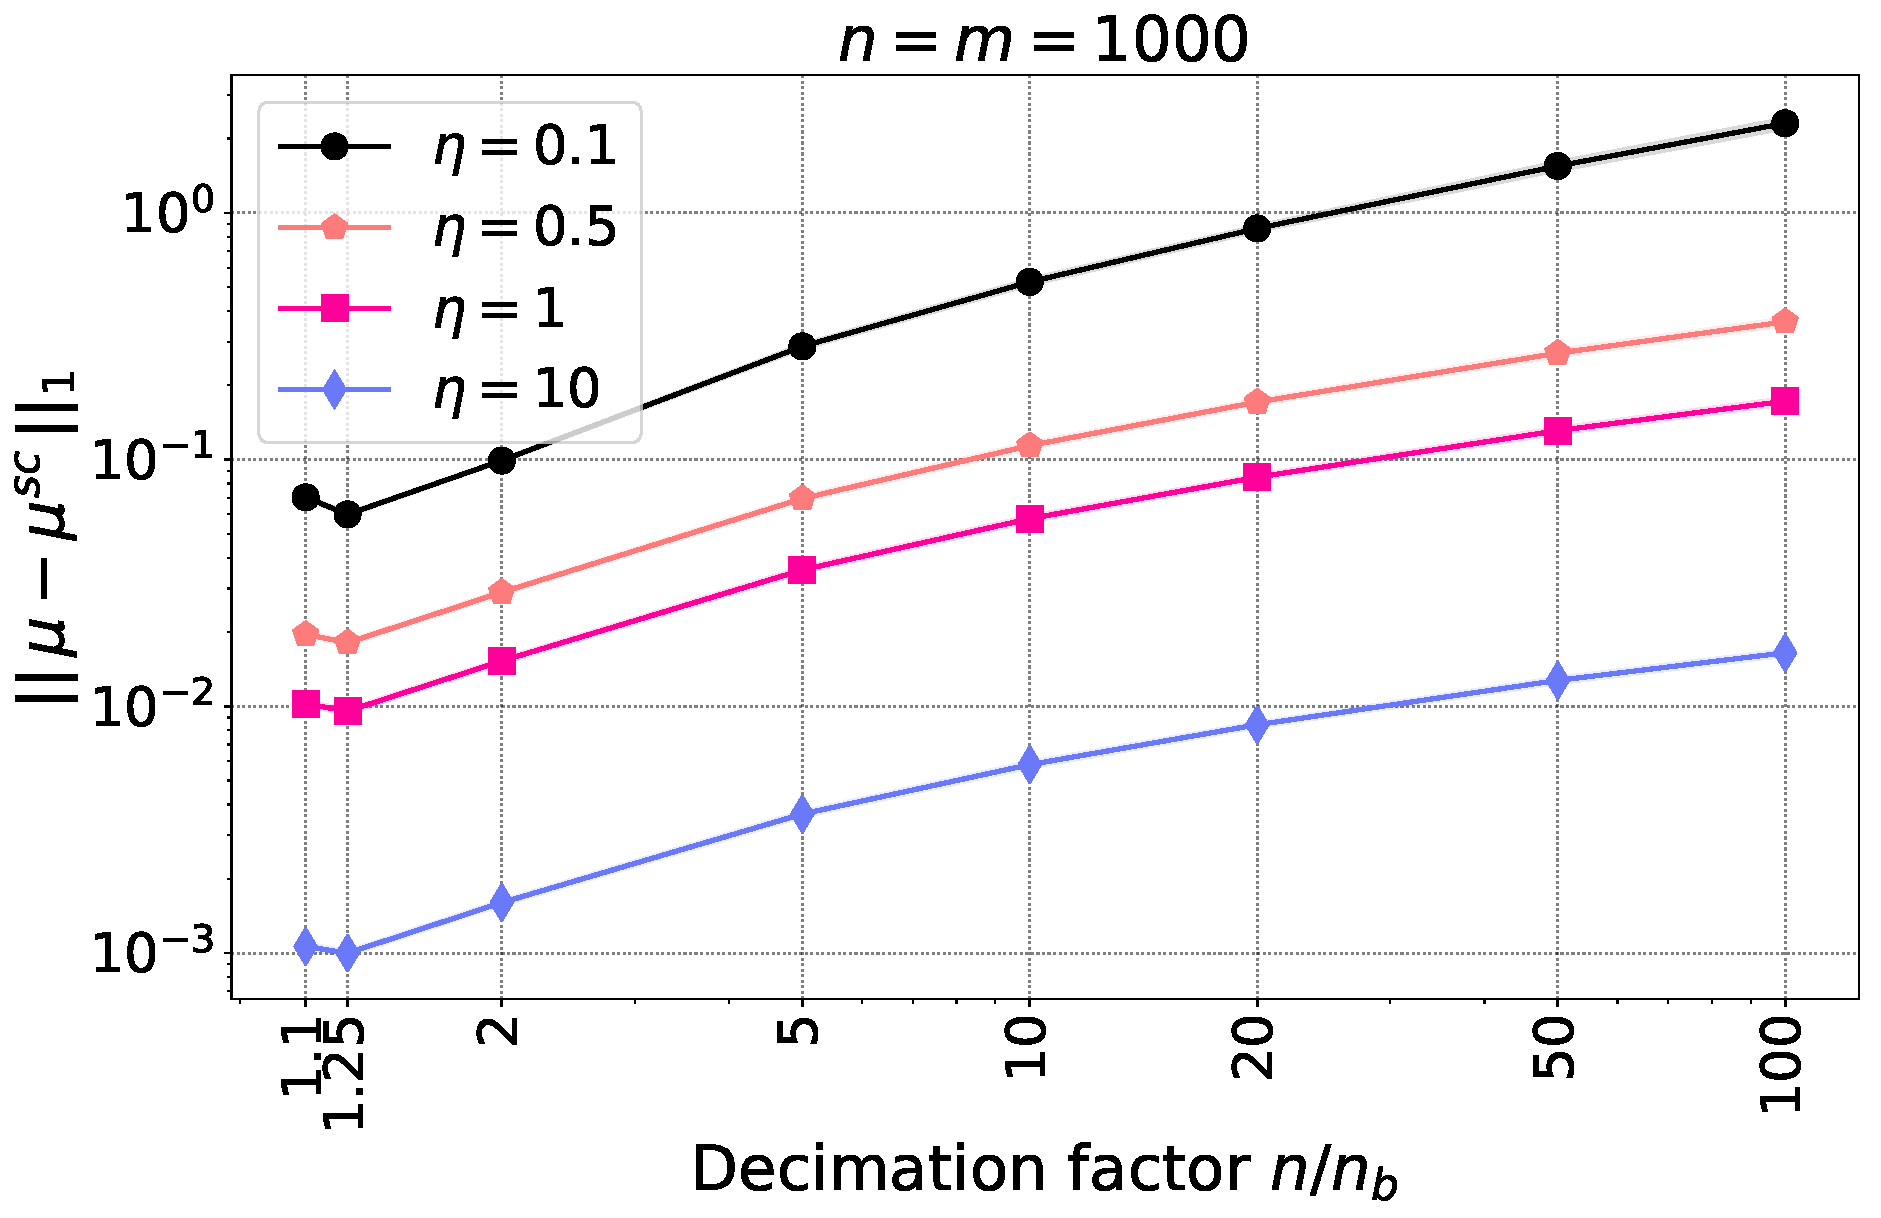
\includegraphics[width=4.55cm]{./figs/norm_M_Mu_marginals_toy_n1000} ~\hfill~
		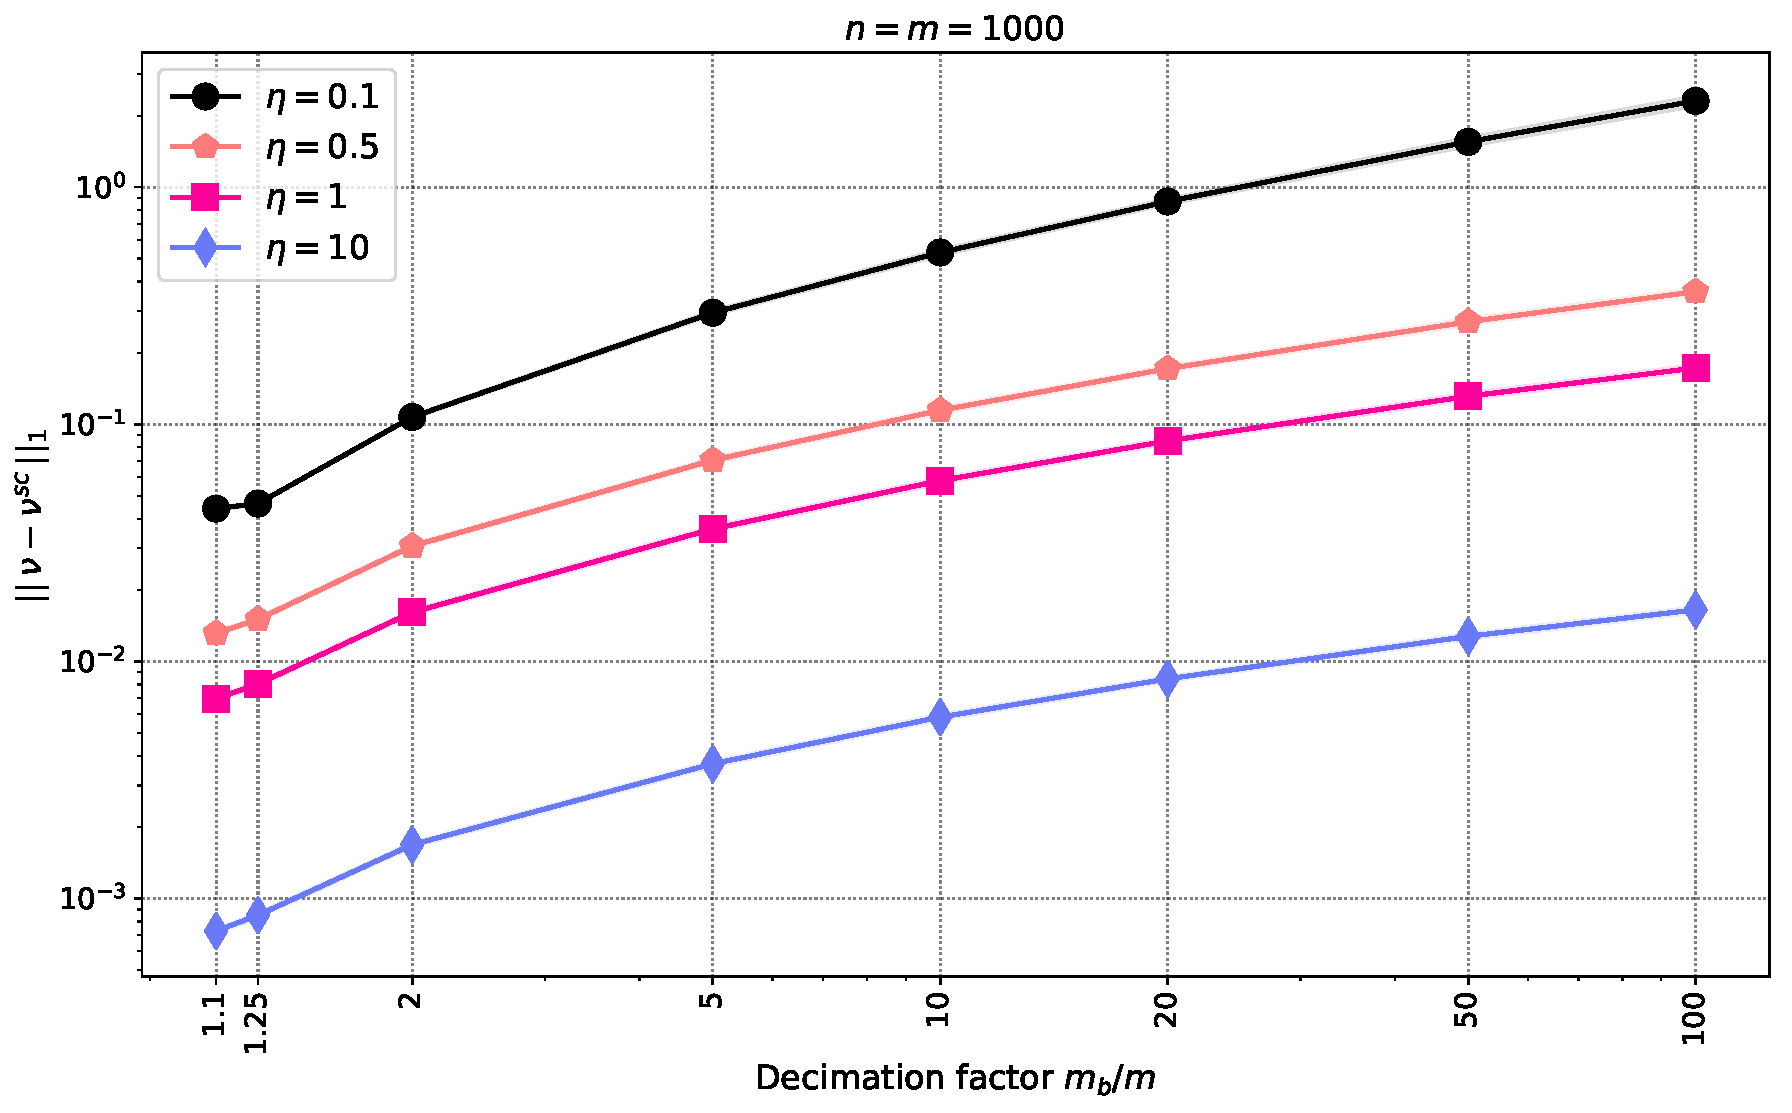
\includegraphics[width=4.55cm]{./figs/norm_M_Nu_marginals_toy_n1000} ~\hfill \\
		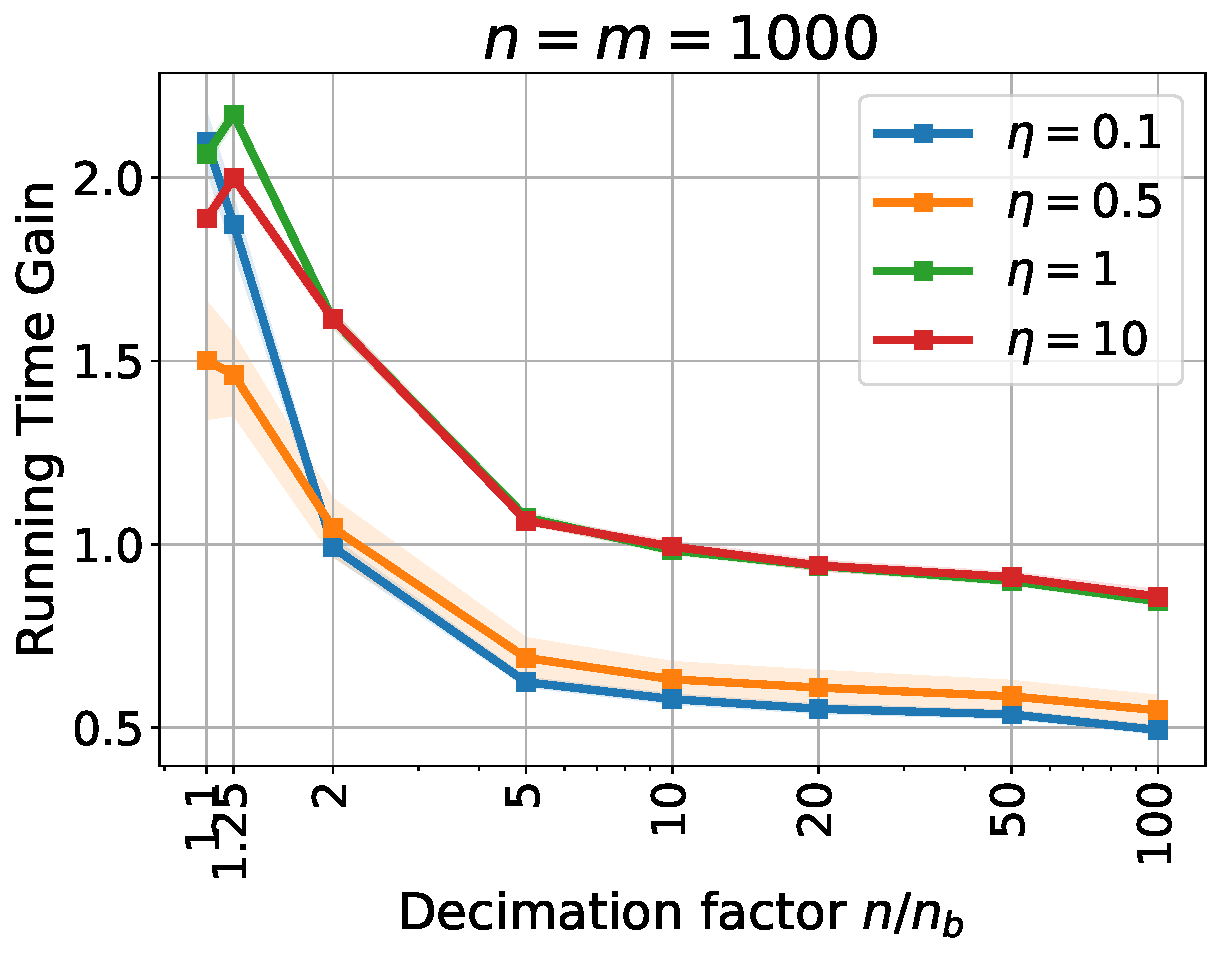
\includegraphics[width=4.55cm]{./figs/norm_M_time_toy_n1000} ~\hfill~
		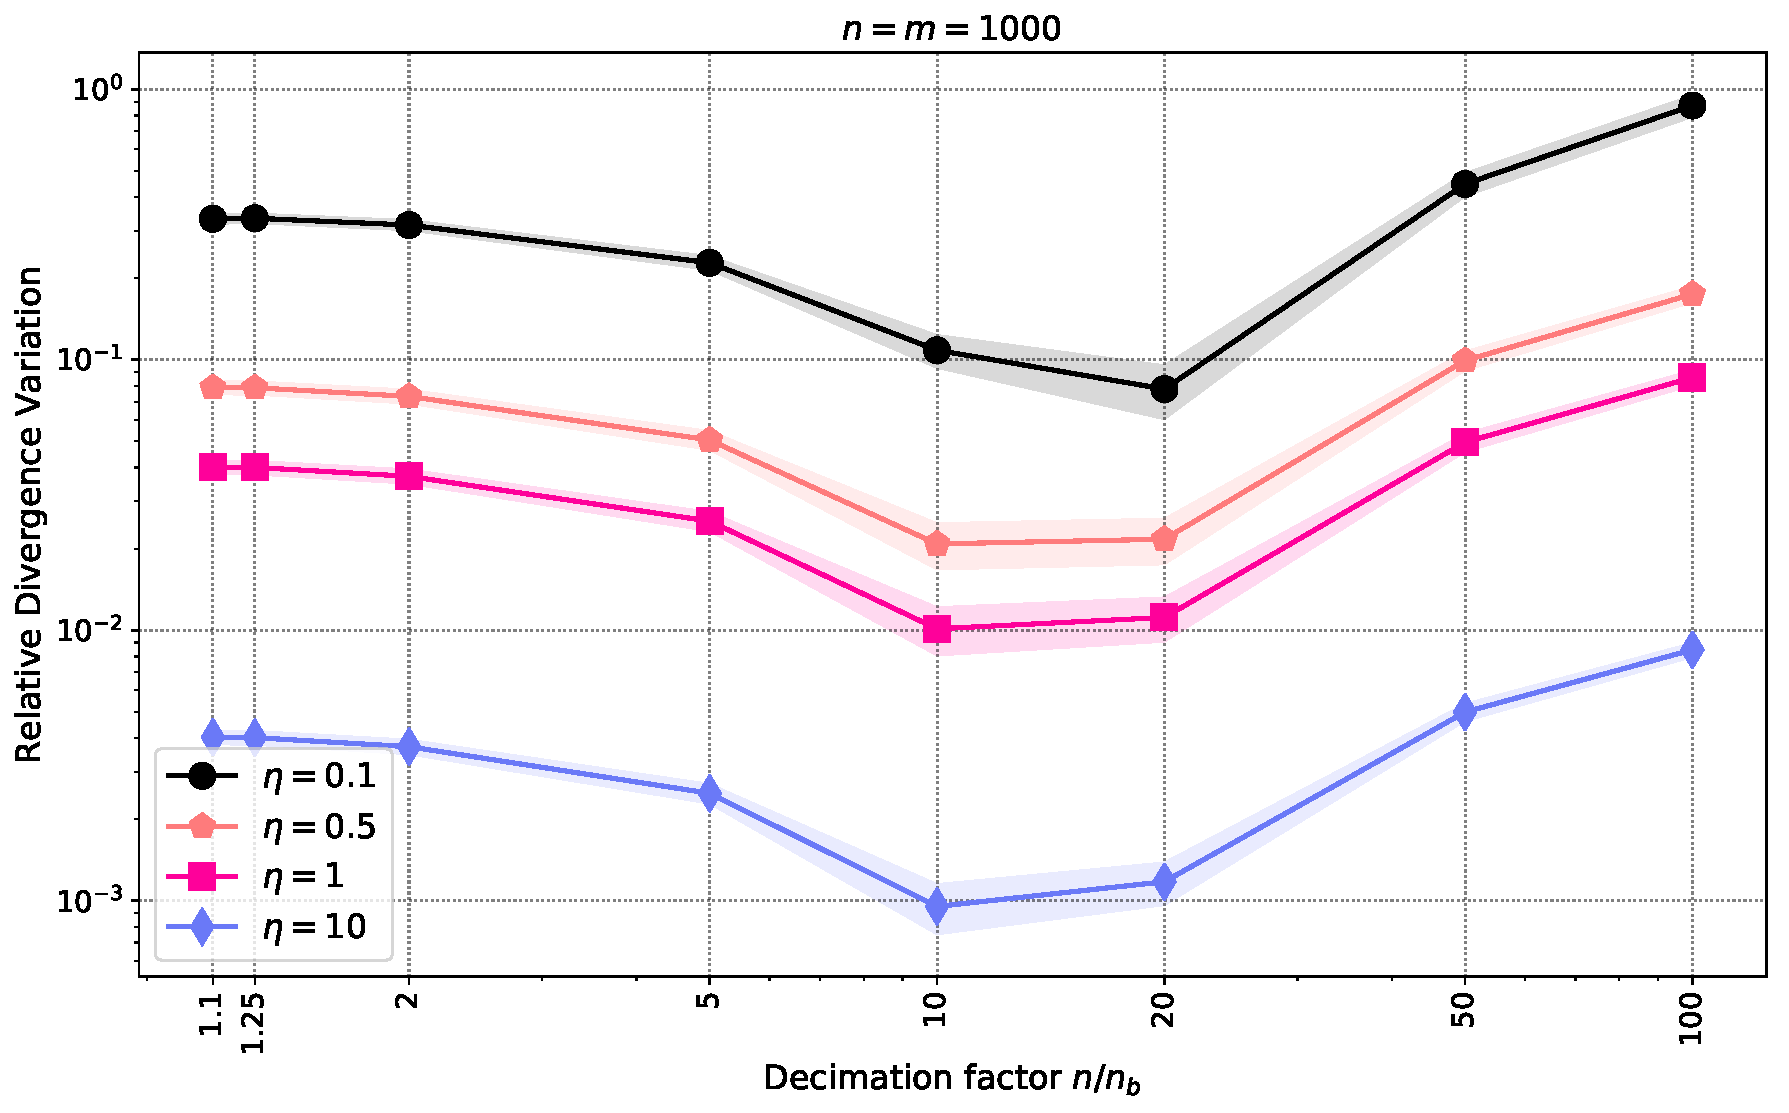
\includegraphics[width=4.55cm]{./figs/norm_M_div_toy_n1000}
	\end{center}
	\caption{Empirical evaluation of \emph{Screenkhorn} vs Sinkhorn for normalized cost matrix. Top panel: marginal violations in relation with the budget of points. Bottom panel: (left) ratio of computation times    $\frac{T_{\text{\emph{Screenkhorn}}}}{T_{\text{Sinkhorn}}}$ and, (right) relative divergence variation. The results are averaged over 10 trials.} 
		\label{fig:margin_expe}
\end{figure*}
%
\emph{Screenkhorn} provides good approximation of the marginals $\mu$ and $\nu$ for ''high'' values of the regularization parameter $\eta$ ($\eta > 1$). The approximation quality diminishes for small $\eta$. As expected $\norm{{\mu} -{\mu}^{\text{sc}}}_1$ and $\norm{{\nu} -{\nu}^{\text{sc}}}_1$ converge towards zero when increasing the budget of points. Remarkably marginal violations are almost negligible whatever the budget for high $\eta$.  According to computation gain, \emph{Screenkhorn} is, up to 2 times, faster than Sinkhorn at low budget $n_b/n$ while the reverse holds when $n_b/n$ gets close to 1.  Computational benefit of \emph{Screenkhorn} also depends on $\eta$ with appropriate values $\eta \leq 1$. Finally except for $\eta=0.1$ \emph{Screenkhorn} achieves a close divergence $\inr{C, P}$ compared to Sinkhorn showing that our static screening test does not harm Sinkhorn divergence.  































\subsection{Integrating \emph{Screenkhorn} into machine learning pipelines}

In this subsection, we analyse the impact of using \emph{Screenkhorn}
instead of Sinkhorn in a complex machine learning pipeline. Our two applications
are a dimensionality reduction technique, denoted as Wasserstein Discriminant Analysis (WDA), based on Wasserstein distance approximated
through Sinkhorn divergence \citep{flamary2018WDA} and a domain-adaptation using optimal transport mapping \citep{courty2017optimal}, named OTDA. 


WDA aims at finding a linear projection which minimize the ratio of distance between intra-class samples and distance inter-class samples, where the distance is understood
in a Sinkhorn divergence sense. We have used a toy problem involving Gaussian classes with $2$ discriminative features and $8$ noisy features and the MNIST dataset. For the
former problem, we aim at find the best two-dimensional linear subspace in a WDA sense whereas for MNIST, we look for a subspace of dimension $20$ starting from the original
$728$ dimensions.  Quality of the retrieved subspace are evaluated using classification task based on a $1$-nearest neighbour approach.

Figure \ref{fig:wda} presents the average gain (over $30$ trials) in computational time we get as the number of examples evolve and for different decimation factors of the \emph{Sinkhorn} problem.
Analysis of the quality of the subspace have been deported to the supplementary material (see Figure \ref{}), but we can remark a small loss of performance of Screenkhorn for the toy problem, while
for MNIST, accuracies are equivalent regardless of the decimation factor.  We can note
that for the minimal gains are respectively $2$ and $4.5$ for the toy and MNIST problem
whereas the maximal gain for $4000$ samples is slightly larger than an order of magnitude. 

\begin{figure*}[t]
	\centering
%	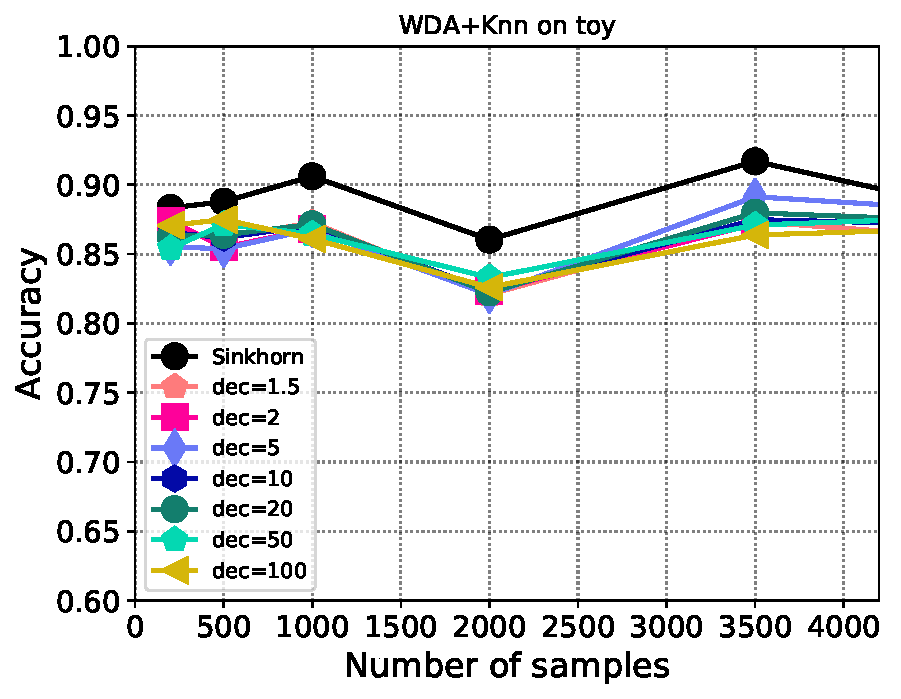
\includegraphics[width=4.cm]{./figs/wda_accur_toy.pdf}
%	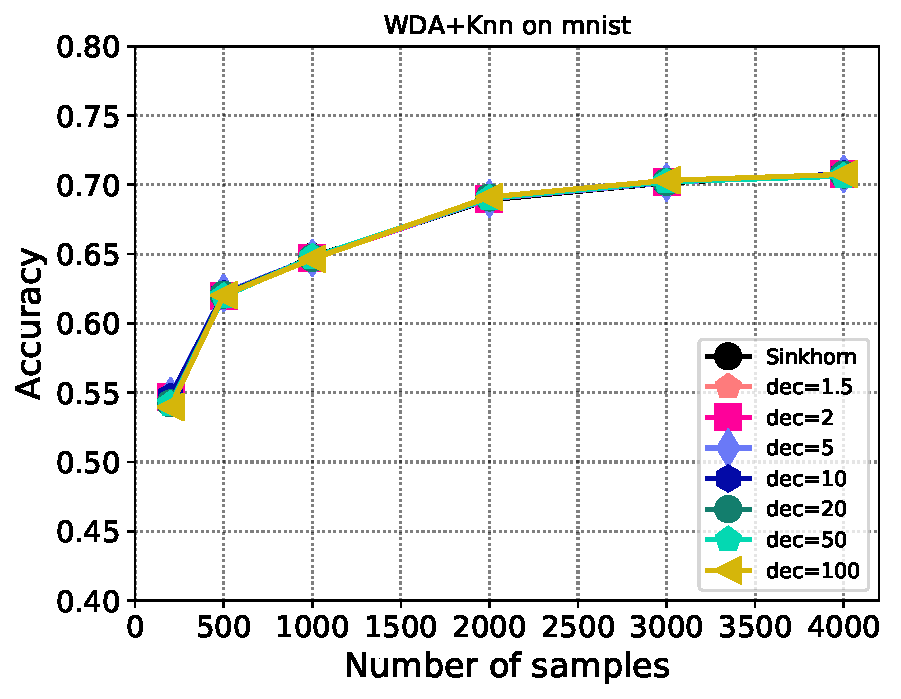
\includegraphics[width=4.cm]{../figs/wda_accur_mnist.pdf}
	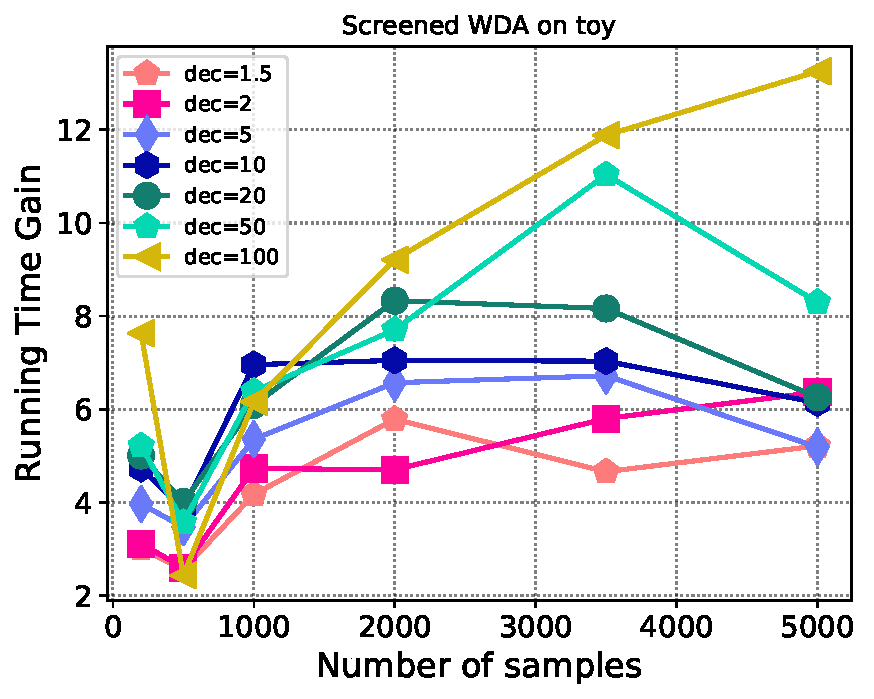
\includegraphics[width=6.cm]{./figs/wda_gain_toy.pdf}
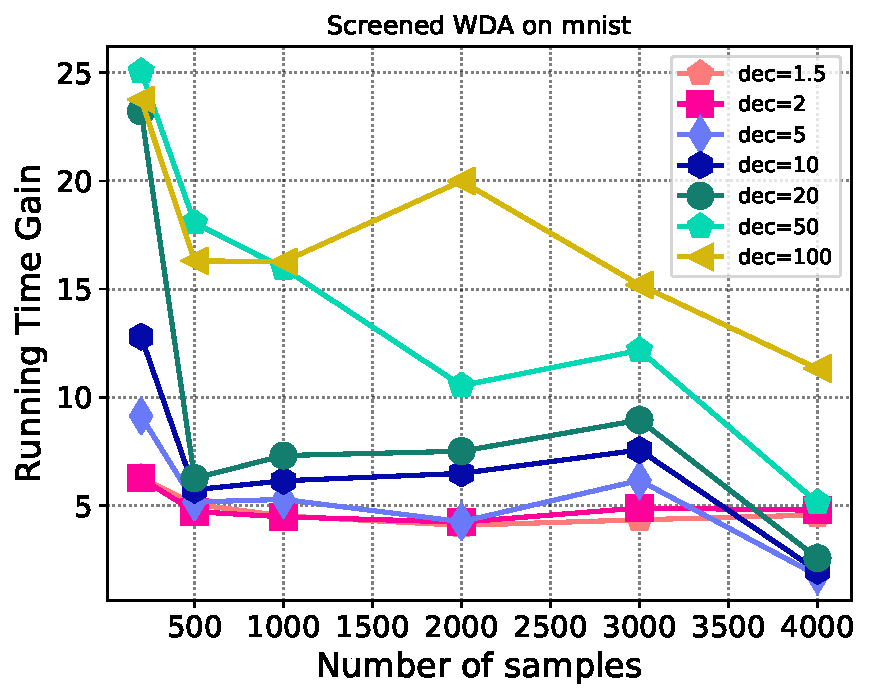
\includegraphics[width=6.cm]{./figs/wda_gain_mnist.pdf}
	\caption{Wasserstein Discriminant Analysis : running time gain for a toy dataset and for mnist as a function of the number of examples and the data decimation factor in \emph{Screenkhorn}}.
	\label{fig:wda}
\end{figure*}
\begin{figure*}[t]
	\centering

	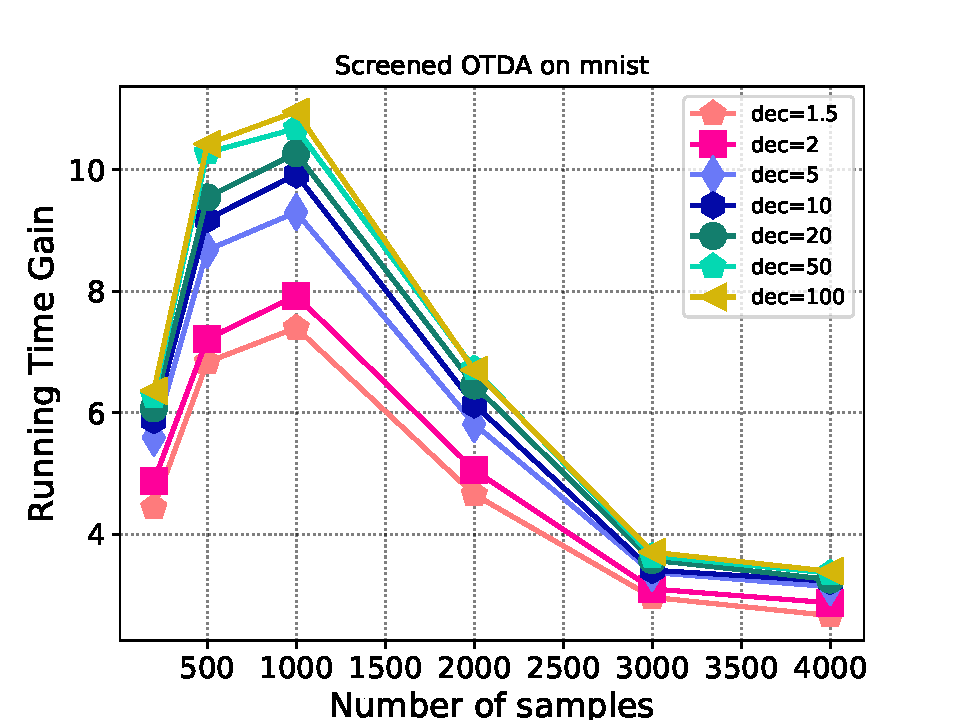
\includegraphics[width=6.cm]{./figs/da_gain_mnist_regcl1.pdf}
	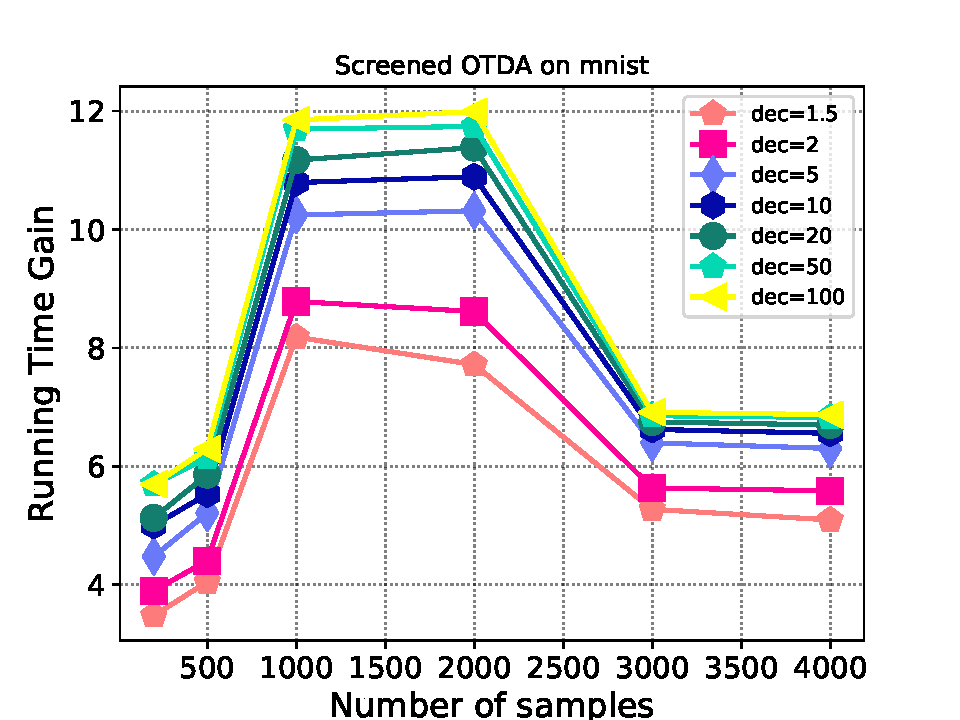
\includegraphics[width=6.cm]{./figs/da_gain_mnist_regcl10.pdf}
	\caption{OT Domain adaptation : running time gain for a toy dataset and for mnist as a function of the number of examples and the data decimation factor in \emph{Screenkhorn}}.
	\label{fig:otda}
\end{figure*}

For the optimal transport based domain adaptation problem, we have considered the
OTDA with $\ell_{0.5,1}$ group-lasso regularizer that helps in exploiting available labels in the source domain. The problem is solved using an majorization-minimization approach 
for handling the non-convexity of the problem. Hence, at each iteration, a Sinkhorn/Screenkhorn has to be computed. As a domain-adaptation problem, we have
used a MNIST to USPS problem in which features have been extracted from the
feature extractor of an domain adversarial neural networks \citep{ganin2016domain} before full convergence of the networks (so as to leave room for OT adaptation). 
Figure \ref{fig:otda} reports the gain in running time for $2$ different values
of the group-lasso regularizer hyperparameter, while the curves of performances are
reported in the supplementary material. We can note that for all the  \emph{Screenkhorn} with different decimation factors, the gain in computation goes from a factor of $4$ to $12$, while accuracies are somewhat equivalent.



% section numerical_experiments (end)